\documentclass[10pt]{beamer}
\usepackage[utf8]{inputenc}
\usepackage{commath}
\usepackage{listings}
\usepackage{xcolor}
\usepackage{array}
\usepackage{makecell}
\usepackage{hyperref}
\hypersetup{
    colorlinks=true,
    linkcolor=blue,
    filecolor=magenta,      
    urlcolor=cyan,
}
\usepackage{amsmath}
\usepackage{amstext}
\usepackage{nccmath}
%\usepackage{showframe}
\usepackage{amssymb} 
\usetheme[progressbar=frametitle]{metropolis}
\usepackage{appendixnumberbeamer}
\usepackage{booktabs}
\usepackage[scale=2]{ccicons}


\lstset{language=Python}
\lstset{frame=lines}
\lstset{caption={Insert code directly in your document}}
\lstset{label={lst:code_direct}}
\lstset{basicstyle=\tiny}
\lstset{basicstyle=\footnotesize}

\lstdefinestyle{cpp}{
  language=C++,
  stepnumber=1,
  numbersep=10pt,
  tabsize=2,
  showspaces=false,
  showstringspaces=false,
  basicstyle=\scriptsize,
  breaklines
}



\usepackage{pgfplots}
\usepgfplotslibrary{dateplot}

\usepackage{xspace}
\newcommand{\themename}{\textbf{\textsc{metropolis}}\xspace}
\newcommand{\ip}[2]{{\langle #1, #2 \rangle}}

\title{User-facing ML or LTR is everywhere}
%\subtitle{Generic algorithms and performance}
% \date{\today}
\date{}
\author{Тарас Шевченко}
\institute{Senior Machine Learning Programmer at Proxet / Giphy}
% \titlegraphic{\hfill\includegraphics[height=1.5cm]{logo.pdf}}
\begin{document}

\maketitle

%\begin{frame}{Table of contents}
%  \setbeamertemplate{section in toc}[sections numbered]
%  \tableofcontents[hideallsubsections]
%\end{frame}


\begin{frame}{Goal}
    Take a popular service and review Machine Learning use-cases.

\begin{figure}
    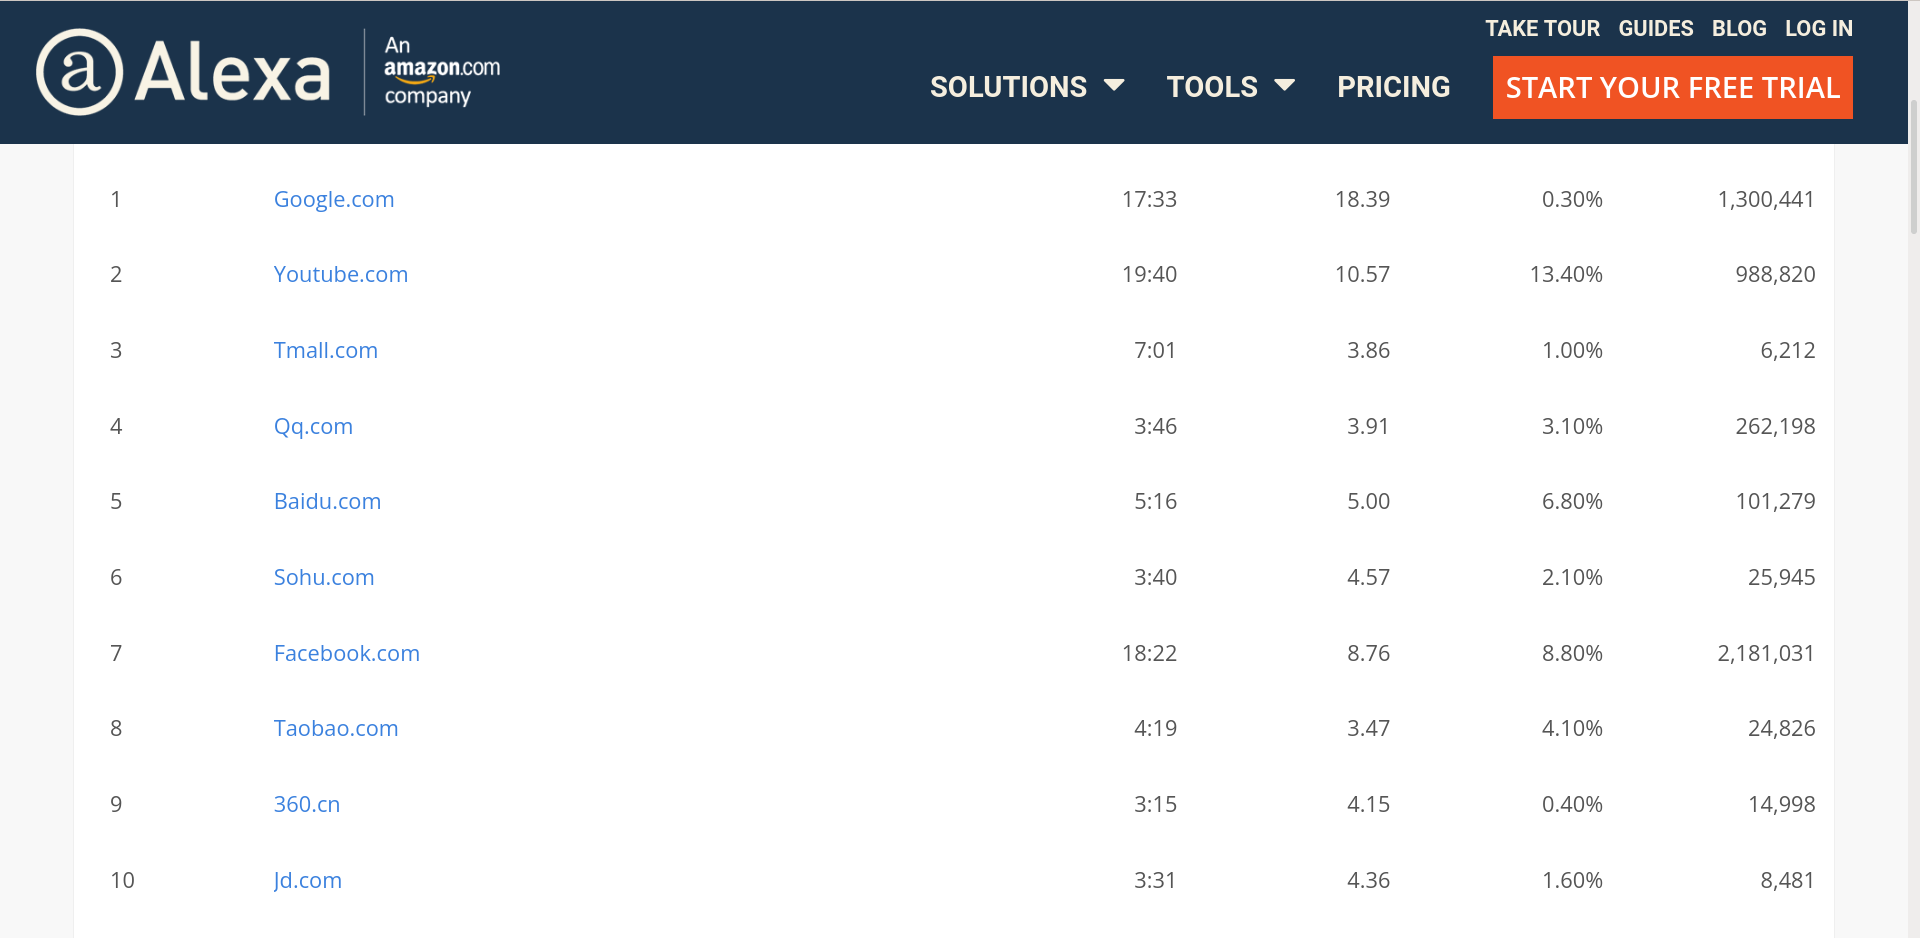
\includegraphics[height=5cm]{images/alexa-top.png}
    \caption{Top websites according to Alex.com}
\end{figure}

\end{frame}


\begin{frame}{Youtube - Home Page after 1 search query}
\begin{figure}
    
\includegraphics[height=5cm]{images/yt-3.png}
\end{figure}
\end{frame}

\begin{frame}{Youtube - Autocomplete}
\begin{figure}
    
\includegraphics[height=5cm]{images/autocomplete.png}
\end{figure}
\end{frame}

\begin{frame}{Youtube - Search}
\begin{figure}
    
\includegraphics[height=5cm]{images/yt-2.png}
\end{figure}
\end{frame}

\begin{frame}{Youtube - Comments}
\begin{figure}
    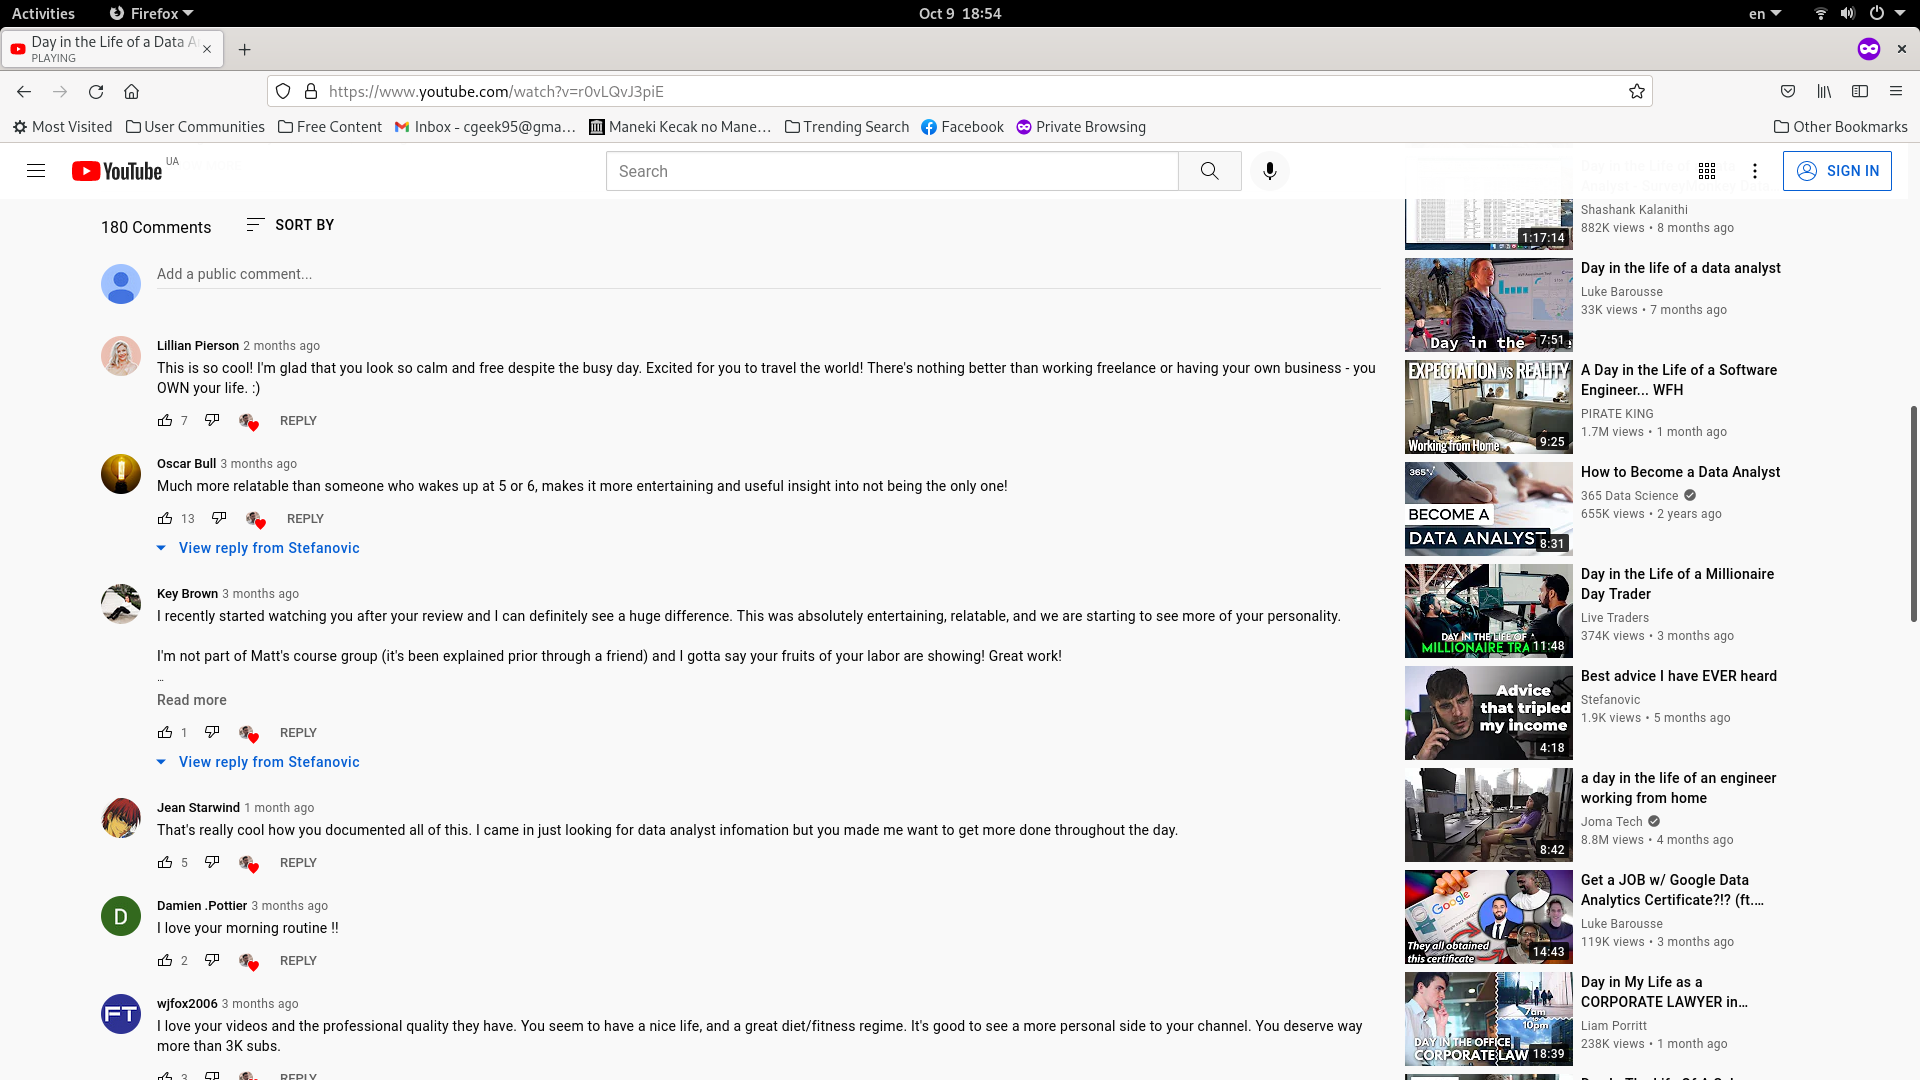
\includegraphics[height=5cm]{images/yt-5.png}
\end{figure}
\end{frame}



\begin{frame}{Classification of Machine Learning Problems [Part 1]}
    \begin{itemize}
        \item Learning Problems
        \item Hybrid Learning Problems
        \item Statistical Inference
        \item Learning Techniques
    \end{itemize}
\end{frame}

\begin{frame}{Classification of Machine Learning Problems [Part 2]}
\begin{figure}
    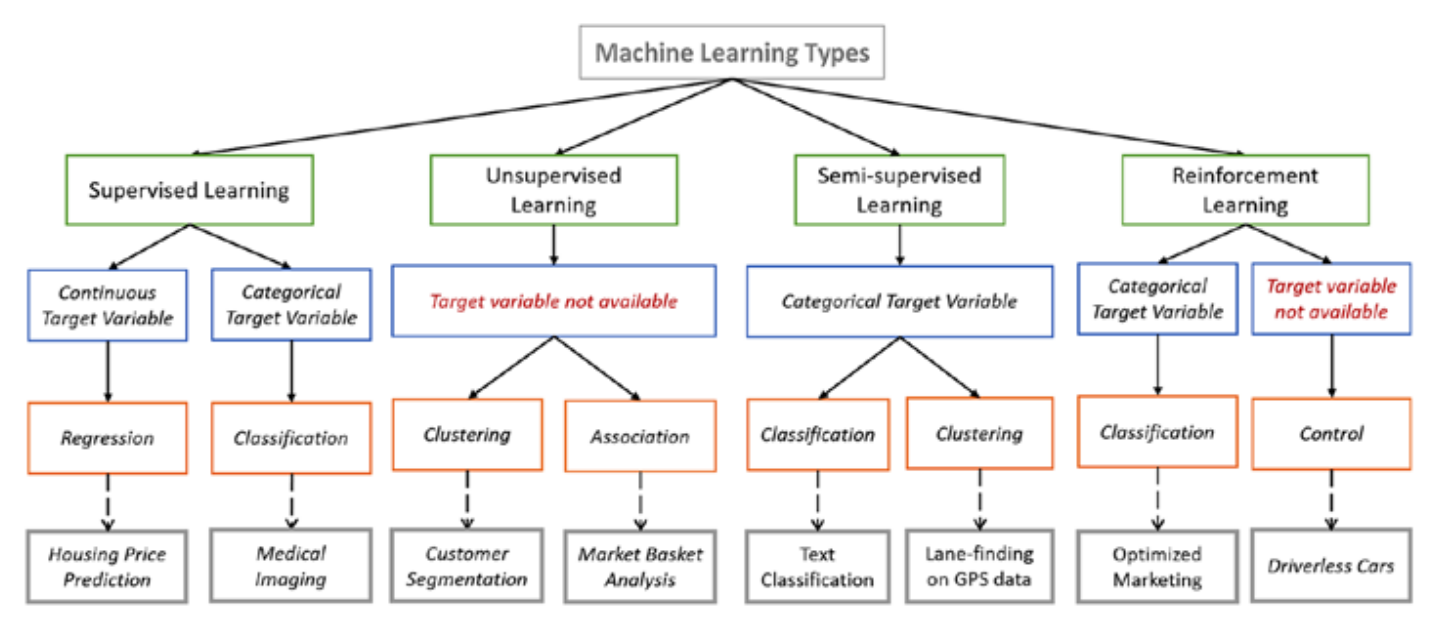
\includegraphics[height=5cm]{images/categorization.png}
    \caption{\href{https://en.proft.me/2015/12/24/types-machine-learning-algorithms/}{Types of Machine Learning Algorithms}}
\end{figure}
\end{frame}


\begin{frame}{Youtube Services}
    \begin{itemize}
        \item {[Personalized]} Home Page Content Selection
        \item {[Personalized]} Global Search
        \item {[Personalized]} Channel Search
        \item {[Personalized]} Search Autocomplete
        \item {[Personalized]} Related Videos
        \item {[Personalized]} Playlists
        \item {[Personalized]} Trending
        \item {[Personalized]} Notifications
        \item {[Personalized]} Comments selection 
        \item Copyright Violation
            \begin{itemize}
                \item By Performer
                \item By Music
                \item By Text
                \item Abusive speech
                \item Violance
            \end{itemize}
        \item {[Personalized]} ADs
        \item Security
    \end{itemize}
\end{frame}

\begin{frame}{Learning to Rank}
        \begin{center}
LTR is everywhere, where we have a list of elements.
    \end{center}
\begin{figure}
    
\includegraphics[height=5cm]{images/learning-to-rank-everywhere.jpg}
\end{figure}
\end{frame}


\begin{frame}{Approaches to Learning to Rank}
    \begin{itemize}
        \item Pointwise (Regression/Classification)
        \item Pairwise (LambdaRank IR-SM, Lambda Rank)
        \item Listwise (Soft Rank, SmoothRank, AdaRank, ListNet, BoltzRank)
    \end{itemize}
\end{frame}

\begin{frame}{LTR-related procedures}
    \begin{itemize}
        \item Candidate Generation
        \item Offline ranking
        \item Online ranking
        \item Data Collection
        \item Data debiasing
        \item A/B testing
    \end{itemize}
\end{frame}


\begin{frame}{What is LTR}
    Learning to rank or machine-learned ranking (MLR) is the application of machine learning, typically supervised, semi-supervised or reinforcement learning, in the construction of ranking models for information retrieval systems

    \begin{itemize}
        \item Candidate Generation
        \item Offline ranking
        \item Online ranking
        \item Data Collection
        \item Data debiasing
        \item A/B testing
    \end{itemize}
\end{frame}


\begin{frame}{Search Dataset - Click-Based}
    \begin{center}
    \begin{tabular}{|l|l|l|l|}
        \hline
        \thead{session\_id} & \thead{query}     & \thead{document\_id} & \thead{relevance} \\ \hline
        1                  & machine learning  & 1                   & 0.0                 \\ \hline
        1                  & machine learning  & 2                   & 0.0                 \\ \hline
        1                  & machine learning  & 3                   & 0.0                 \\ \hline
        1                  & machine learning  & 4                   & 0.0                 \\ \hline
        1                  & machine learning  & 5                   & 1.0                 \\ \hline
    \end{tabular}
    \end{center}
\end{frame}

\begin{frame}{Search Dataset - Click-Based}
    \begin{center}
    \begin{tabular}{|l|l|l|l|l|}
        \hline
        \thead{session\_id} & \thead{query}     & \thead{document\_id} & \thead{relevance} & \thead{position} \\ \hline
        1                  & machine learning  & 1                   & 0.0                 & 1 \\ \hline
        1                  & machine learning  & 2                   & 0.0                 & 2 \\ \hline
        1                  & machine learning  & 3                   & 0.0                 & 3 \\ \hline
        1                  & machine learning  & 4                   & 0.0                 & 4 \\ \hline
        1                  & machine learning  & 5                   & 1.0                 & 5 \\ \hline
    \end{tabular}
    \end{center}
\end{frame}



\begin{frame}{Search Dataset - Human Relevance}
    \begin{center}
    \begin{tabular}{|l|l|l|l|}
        \hline
        \thead{session\_id} & \thead{query}     & \thead{document\_id} & \thead{relevance} \\ \hline
        1                  & machine learning  & 1                   & 3.0                 \\ \hline
        1                  & machine learning  & 2                   & 2.0                 \\ \hline
        1                  & machine learning  & 3                   & 1.0                 \\ \hline
        1                  & machine learning  & 4                   & 4.0                 \\ \hline
        1                  & machine learning  & 5                   & 5.0                 \\ \hline
    \end{tabular}
    \end{center}
\end{frame}

\begin{frame}{LTR evaluation}
\begin{equation}
    PairAccuracy = \sum_{i < j}{[rel_{i} > rel_{j}]}
\end{equation}
\begin{equation}
    {\displaystyle \mathrm {DCG_{p}} =\sum _{i=1}^{p}{\frac {rel_{i}}{\log _{2}(i+1)}}}
\end{equation}
\begin{equation}
    {\mathrm  {DCG_{{p}}}}=\sum _{{i=1}}^{{p}}{\frac  {2^{{rel_{{i}}}}-1}{\log _{{2}}(i+1)}}
\end{equation}
\begin{equation}
    {\mathrm  {nDCG_{{p}}}}={\frac  {DCG_{{p}}}{IDCG_{{p}}}}
\end{equation}
\begin{equation}
    {\text{MRR}}={\frac  {1}{|Q|}}\sum _{{i=1}}^{{|Q|}}{\frac  {1}{{\text{rank}}_{i}}}.\!
\end{equation}
\end{frame}

\begin{frame}{CatBoost Training}
\lstinputlisting[language=Python,caption=Train CatBoost LTR with YetiRankPairwise loss]{code/l0.py}
\end{frame}

\begin{frame}{LTR training protocols}
\begin{enumerate}
    \item split by query
    \item backtesting
\end{enumerate}
\end{frame}


\begin{frame}{Clicks vs Explicit feedback}
\begin{enumerate}
    \item Explicit feedback is not vulnerable to spam.
    \item Explicit feedback can be outdated.
    \item Explicit feedback has biases, which you can control with a user's manual.
    \item Explicit feedback has fewer contradictions, but almost all the time, the size of a dataset is much smaller..
    \item You must mimic query distribution in your dataset.
    \item When you start a new product, you don't have enough clicks.
    \item Explicit feedback is expensive, and you have to update the test questions very often.
\end{enumerate}
\end{frame}


\begin{frame}{Search Dataset - Feature Space}
    \begin{enumerate}
        \item $f_1(document\_id)$ - knows about document modalities
        \item $f_2(session\_id)$ - knows about user id, location, previous actions
        \item $f_3(query)$
        \item $f_4(query, document\_id)$
        \item $f_5(query, session_id)$
        \item $f_6(session\_id, document\_id)$
    \end{enumerate}
\end{frame}


\begin{frame}{Search Dataset - Feature Examples}
    \begin{enumerate}
        \item textual similarity (BM25, BM25 + Stemming, vector-space models)
        \item document-level CTR from search logs
        \item document-level CTR from recommendations logs
        \item different counter aggregations
        \item Word2Vec on clicks (StartSpace implementation)
        \item 'PageRank'
        \item fraud detection
        \item OCR + textual similarity
        \item speach recongntion + textual similarity
    \end{enumerate}
    The gradient boosting with YetiRankPairwise loss function gives the best results. Neural Nets are not as good, but you can build a lot of great features with Siamese neural networks. You can get ideas from Question-Answering models. Pinterest uses a simple Convolutional Neural Net, but they haven't tried the CatBoost with YetiRankPairwise loss.
\end{frame}

\begin{frame}{Search Dataset - Data Colection}
You need at least two table:
    \begin{enumerate}
        \item Requests and Responses (timestamp, query, document\_id, position, response\_id, location, user\_id, device\_id, session\_id)
        \item Actions (timestamp, response\_id, action\_id, document\_id)
    \end{enumerate}
You can use Column-oriented database and a queue like kafka to collect the logs. Also, you can duplicate the data on S3.
\end{frame}


\begin{frame}{Personalization}
    \begin{itemize}
        \item you can train different models for different regions or encode a location in your features
        \item you can have different search algorithm for different user buckets
        \item user-based personalization kills caching 
        \item you can cache heavy features from the head of your search log
    \end{itemize}
\end{frame}


\begin{frame}{Search vs Recommentations}
\begin{itemize}
    \item almost identical approach is applicable for Recommendation Systems, but the document id plays the role of a query.
    \item you should reuse document-level features
    \item you can recompute the same feature, but on different datasets
    \item recommentations are almost identical to search, but for relatively small collections you can use a heavy artillery, because you can store predictions in a relatively small matrix
    \item you can use top search predictions to generate recommendations
\end{itemize}
\end{frame}


\begin{frame}{LTR for every product}
    \begin{center}
    \begin{tabular}{|l|l|l|l|l|}
        \hline
        \thead{Task}            & \thead{Query} & Document             & \thead{Personalizable} & \thead{A/B  test \\ Target} \\ \hline
        \makecell{Search}                  & Query String  & \makecell{Document \\ Id}          & +                      & CTR/MRR \\ \hline
        \makecell{Recommentations}         & Document Id   & \makecell{Document \\ Id}          & +                      & CTR/MRR \\ \hline
        \makecell{Home Page \\ Documents}     & DateTime      & \makecell{Document \\ Id}          & +                   & CTR/MRR  \\ \hline
        \makecell{Home Page \\ Queries}      & DateTime      & \makecell{Query \\ String}         & +                    & CTR/MRR \\ \hline
        \makecell{Search \\ Autocomplete}     & Query String  & \makecell{Query \\ String}         & +                   & CTR/MRR \\ \hline
        \makecell{Ranking \\ Comments}        & Document Id   & \makecell{Comment \\ + \\ Metadata}   & +  & Likes \\ \hline
    \end{tabular}
    \end{center}
\end{frame}



\begin{frame}{Materials}
\begin{enumerate}
    \item \href{https://static.googleusercontent.com/media/guidelines.raterhub.com/en//searchqualityevaluatorguidelines.pdf}{Search Quality Rating Guidelines}
    \item \href{https://nlp.stanford.edu/IR-book/information-retrieval-book.html}{Introduction to Information Retrieval}
    \item \href{https://www.amazon.com/Information-Retrieval-Implementing-Evaluating-Engines/dp/0262528878}{Information Retrieval: Implementing and Evaluating Search Engines}
    \item \href{https://arxiv.org/pdf/1803.09799.pdf}{Demystifying Core Ranking in Pinterest Image Search}
    \item \href{https://github.com/catboost/tutorials/blob/master/ranking/ranking_tutorial.ipynb}{Catboost usage example.}
    \item \href{https://github.com/facebookresearch/StarSpace.git}{StarSpace}
    \item \href{https://www.microsoft.com/en-us/research/wp-content/uploads/2016/08/fp073-wu.pdf}{Personalized Trending Search Suggestions}
    \item \href{http://proceedings.mlr.press/v14/gulin11a/gulin11a.pdf}{Winning The Transfer Learning Track of Yahoo!’s Learning To Rank Challenge with YetiRank}
    \item \href{https://www.cs.cmu.edu/~pradeepr/paperz/ndcg.pdf}{On NDCG Consistency of Listwise Ranking Methods}
    \item \href{https://dl.acm.org/doi/abs/10.1145/2996913.2996986}{GeoTrend: Spatial Trending Queries on Real-time Microblogs}
    \item \href{https://dl.acm.org/doi/abs/10.1145/2339530.2339594}{Finding Trending Local Topics in Search Queries}
    \item \href{https://research.google/pubs/pub37797/}{Challenges in building large-scale information retrieval systems: invited talk}
    \item \href{http://stepanovpapers.com/SIMD_Decoding_TR.pdf}{SIMD-Based Decoding of Posting Lists}
\end{enumerate}
\end{frame}


\end{document}
